\section{研究背景与范围}

BaZn$_2$Si$_2$O$_7$ 是 BaO--ZnO--SiO$_2$ 体系中具有可逆结构转变的硅酸盐。其低温相表现出显著正热膨胀，而加热后形成的高温相可呈近零或负热膨胀，因而成为研究四面体链柔性和组成调控的模型体系。Lin 等通过高温衍射解析了相变及两种晶体结构，是后续相控制研究的结构基准 \cite{lin1999phase}。

本综述围绕三个问题展开：第一，BaZn$_2$Si$_2$O$_7$ 的结构和合成条件如何共同决定主相；第二，Ba/Sr、Zn/Mg/Co/Ni/Cu 和 Si/Ge 替位能够在多大范围内迁移相稳定性；第三，Ba$_5$Y$_{12}$Zn[O(SiO$_4$)]$_8$ 作为结构类似物的说法有哪些可核查依据。公开数据库可确认 BaZn$_2$Si$_2$O$_7$ 的正交结构、Ba 的五配位以及 ZnO$_4$ 与 SiO$_4$ 四面体的角共享网络 \cite{available2020materials}，但本次检索未找到 Ba$_5$Y$_{12}$Zn[O(SiO$_4$)]$_8$ 的可核验晶体学原始论文。因此，文中将“直接报道”“近邻体系”和“结构推断”严格分开。

近邻体系并非附属背景。Ba$_{1-x}$Sr$_x$Zn$_2$Si$_2$O$_7$ 的研究表明，少量 Sr 替位即可稳定高温结构至室温，并把热膨胀系数调到负值区间 \cite{thieme2015ba1,thieme2016very}；Zn 位的异价或等价替位则进一步改变相变温度和各向异性 \cite{thieme2016new,kerstan2013bazn2si2o7}。这些结果为目标类似物的比较提供了可迁移的结构—工艺语言，但不等价于 Ba$_5$Y$_{12}$Zn[O(SiO$_4$)]$_8$ 已经被合成。

图~\ref{fig:roadmap} 给出全文推进顺序，图~\ref{fig:taxonomy} 将结构、合成、相控制和证据边界放在同一框架中。

\begin{figure}[t]
  \centering
  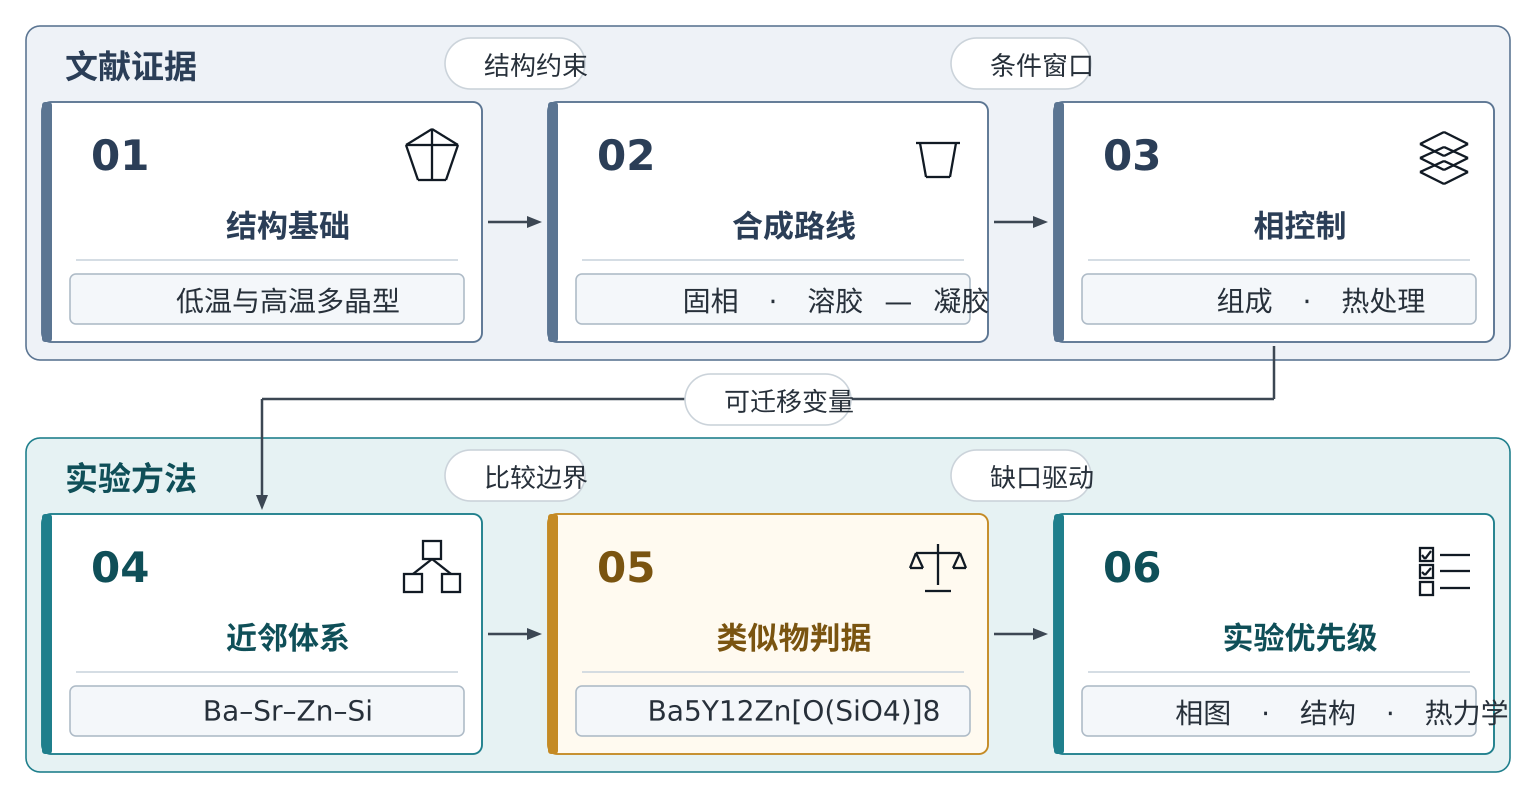
\includegraphics[width=\linewidth]{../figures/svg/roadmap_bazn2si2o7.svg}
  \caption{本文的行文路线图。箭头表示从结构事实到合成窗口、近邻迁移和可证伪实验建议的推进顺序。}
  \label{fig:roadmap}
\end{figure}
